\documentclass{article}

\usepackage[legalpaper, margin=1in]{geometry}
\usepackage{url}
\usepackage{booktabs}
\usepackage{amsmath}
\usepackage{graphicx}
\usepackage{chngcntr}
\usepackage{hyperref}
\usepackage{booktabs}
\usepackage{tabularx}
\usepackage{subfig}
\usepackage{longtable}
\usepackage{dblfloatfix}
\usepackage{listings}
\usepackage{placeins}
\usepackage{float}
\usepackage[dvipsnames]{xcolor}
\usepackage[style=ieee]{biblatex}

\addbibresource{refs.bib}
\DeclareCiteCommand{\citetitle}
{\boolfalse{citetracker}%
	\boolfalse{pagetracker}%
	\usebibmacro{prenote}}
{\ifciteindex
	{\indexfield{indextitle}}
	{}%
	\printtext[bibhyperref]{\printfield[citetitle]{labeltitle}}}
{\multicitedelim}
{\usebibmacro{postnote}}

\counterwithin{figure}{section}
\hyphenation{op-tical net-works semi-conduc-tor}


\begin{document}

\newcommand{\titleName}{Midterm - Design of a Heat Exchanger}
\newcommand{\courseName}{ME-407: Computational Fluid Dynamics}
\newcommand{\dateCreated}{\today}
\newcommand{\professorName}{Professor Bondi}

\begin{titlepage}
	\newcommand{\HRule}{\rule{\linewidth}{0.5mm}}
	\center
	\textsc{\LARGE Cooper Union for the Advancement of Science and
		Art}\\[1.5cm]
	{\color{teal} \HRule\\[0.4cm]}
	{\huge\bfseries \titleName\\[0.5cm] \textmd{\LARGE \courseName}}\\[0.4cm]
	{\color{teal} \HRule\\[0.4cm]}
	\begin{minipage}{0.4\textwidth}
		\begin{flushleft}
			\large
			\textit{Authors:}\\
			\textsc{Michal Meiner} \\
			\textsc{Preston Xu} \\
			\textsc{Benjamin Meiner} \\
			\textsc{Neil Sawhney} \\
		\end{flushleft}
	\end{minipage}
	~
	\begin{minipage}{0.4\textwidth}
		\begin{flushright}
			\large
			\textit{Professor:}\\
			\textsc{\professorName}

		\end{flushright}
	\end{minipage}
	\vfill\vfill\vfill
	{\large\dateCreated}
	\vfill
	%----------------------------------------------------------------------------------------

	\newpage
	\tableofcontents
\end{titlepage}

\title{\titleName}

%%%%%%%%%%%%%%%%%%%%%%%%%%%%%%%%%%%%%%%%%%%%%%%%%%%
%%%%%%%%%%%%%%%%%%%%%%%%%%%%%%%%%%%%%%%%%%%%%%%%%%%
\section{Objective}
% The objective of this assignment is to utilize Fluent to determine the effects of different turbulence models on a CFD simulation of low around a blunt object. The object to be simulated is a 3d block in the middle of a square channel as shown in \autoref{fig:problem}. The block and channel have the following dimensions:
% \begin{itemize}
% 	\item Obstruction cross section: 25mm x 25mm, centered in channel.
% 	\item Cross section of channel: 150mm x 150mm.
% 	\item Pre obstruction channel length: 1m or minimum required to obtain a fully developed flow profile before the obstruction.
% 	\item Post obstruction channel length: 3m or minimum required to prevent backflow.
% \end{itemize}

% \begin{figure}[h]
% 	\centering
% 	\includegraphics[width=0.5\linewidth]{img/problem.png}
% 	\caption{Geometry Scheme}
% 	\label{fig:problem}
% \end{figure}

% The separation and flow pattern of the air near the beginning of the obstruction will be calculated. Specifically the following will be determined:
% \begin{itemize}
% 	\item The length before reattachment occurs.
% 	\item The pressure drop for the last 4m of the channel.  The calculations should be performed using the following turbulence models:
% 	\item Spalart-Allmaras
% 	\item Standard $k-\epsilon$
% 	\item Realizable $k-\epsilon$ model
% 	\item SST $k-\omega$ model
% 	\item Reynolds Stress Model
% \end{itemize}

%%%%%%%%%%%

\subsection{Model Assumptions}

% \begin{itemize}
% 	\item Because the Reynolds number is high at 50,000, the flow is assumed to be turbulent.
% 	\item Because the flow is symmetric, only a quarter of the geometry will be modeled.
% \end{itemize}

%%%%%%%%%%%%%%%%%%%%%%

\section{Ballpark Hand Calculations}
To verify the CFD results to follow, ballpark hand calculations must be performed.

%%%%%%%%%%%

\subsection{Inlet Duct}

%%%

\subsubsection{Velocity Drop Over the Length of the Model}
The minimum velocity of 20 mph will be used at the inlet to ensure the worst case scenario is considered.

If we assume the flow is incompressible we can use conservation of mass to calculate the output velocity as shown in \autoref{eq:velocity-inlet_duct}. Because the inlet area is equal to the outlet area, the average velocity at the outlet is equal to the velocity at the inlet.

\begin{equation}
	\begin{aligned}
		A_1 V_1  & = A_2 V_2             \\
		V_2      & = \frac{A_1 V_1}{A_2} \\
		         & = \frac{A_1 V_1}{A_1} \\
		         & = V_1                 \\
		\Delta V & = 0
	\end{aligned}
	\label{eq:velocity-inlet_duct}
\end{equation}

%%%

\subsubsection{Pressure Drop Over the Length of the Model}

From the Darcy-Weisbach equation\cite{professional_engineer} the frictional head loss across the duct is given by \autoref{eq:darcy_weisbach}
\begin{equation}
	h_f = \frac{f L V^2}{2gD}
	\label{eq:darcy_weisbach}
\end{equation}

where
\begin{quote}
	\begin{description}
		\item[$f$] = the Moody, Darcy, or Stanton friction factor and is a function of $Re$ and $\frac{\epsilon}{D}$
		\item[$D$] = hydraulic diameter of the duct
		\item[$L$] = length over which the pressure drop occurs
		\item[$g$] = acceleration due to gravity
		\item[$\epsilon$] = roughness factor for the duct
	\end{description}
\end{quote}

\begin{figure}[h]
	\centering
	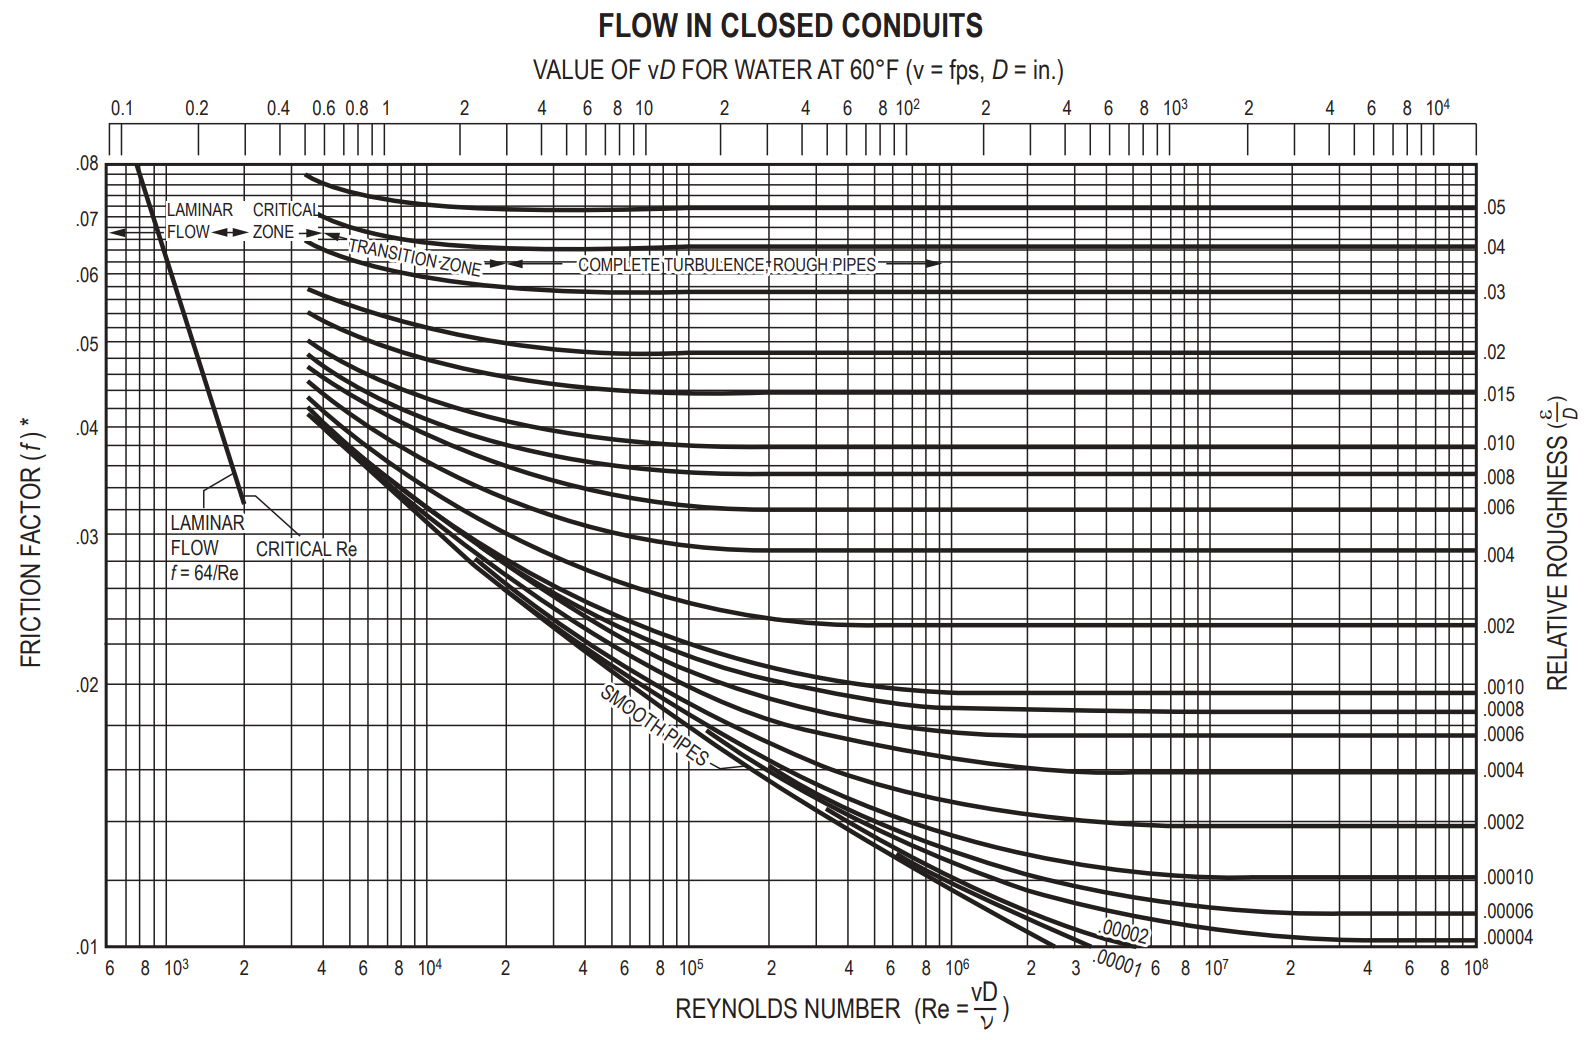
\includegraphics[width=0.5\linewidth]{img/hand_calcs/moody_diagram.png}
	\caption{Moody Diagram from \citetitle{professional_engineer}}
	\label{fig:moody_diagram}
\end{figure}

To find the friction factor, the Reynolds number must be calculated using \autoref{eq:reynolds-inlet_duct}. However, because the cross-section is not circular the hydraulic diameter must be calculated as shown in \autoref{eq:hydraulic_diameter}.

\begin{equation}
	\begin{aligned}
		D_h & = \frac{4A}{P}                                    \\
		    & = \frac{4*(10 in)*(20 in)}{2*(10 in) + 2*(20 in)} \\
		D_h & = 13.333 in
	\end{aligned}
	\label{eq:hydraulic_diameter}
\end{equation}

Now the Reynolds number can be calculated using \autoref{eq:reynolds-inlet_duct}. The density and dynamic viscosity of air at the worst case temperature of 108 $^\circ F$ is 0.070 lb/ft$^3$ and $0.01918$ cP respectively according to \citetitle{engineering_toolbox}.

\begin{equation}
	\begin{aligned}
		Re & = \frac{\rho V D}{\mu}                                      \\
		   & = \frac{(0.070 lb/ft^3)*(20 mph)*(13.333 in)}{(0.01918 cP)} \\
		Re & = 177014.265
	\end{aligned}
	\label{eq:reynolds-inlet_duct}
\end{equation}

The friction factor can now be found using the Moody chart from the \citetitle{professional_engineer} as shown in \autoref{fig:moody_diagram}. The pipe is assumed to be perfectly smooth, which yields a friction factor of 0.016. The pressure drop can then be calculated using \autoref{eq:pressure_drop}. Importantly, the friction factor assumes that the flow is fully developed, which it is not in this case. However, the pressure drop is only being used as a ballpark figure to compare to the CFD results, so this assumption is acceptable.

The head loss due to friction is then calculated using \autoref{eq:head_loss-inlet_duct} where the length over which the pressure drop occurs is measured from the center path line of the geometry to be 66.648 in.

\begin{equation}
	\begin{aligned}
		h_f & = \frac{f L V^2}{2D}                                                 \\
		    & = \frac{0.016*(66.648 in)*(20 mph)^2}{2*(32.174 ft/s^2)*(13.333 in)} \\
		h_f & = 12.834 in
	\end{aligned}
	\label{eq:head_loss-inlet_duct}
\end{equation}

The minor losses from the bend will also be considered. The head loss due to the bend is given by \autoref{eq:head_loss-bend}. The loss factor $K$ is obtained from \citetitle{engineering_toolbox} to be 0.5 for a 45$^\circ$ rounded bend. Although the bend is only 30$^\circ$, using the loss factor for a 45$^\circ$ bend will give a more conservative estimate.

\begin{equation}
	\begin{aligned}
		h_b & = K \frac{V^2}{2g}                         \\
		    & = 0.5 \frac{(20 mph)^2}{2*(32.174 ft/s^2)} \\
		h_b & = 80.23 in
	\end{aligned}
	\label{eq:head_loss-bend}
\end{equation}

The pressure drop is then calculated using \autoref{eq:pressure_drop}.

\begin{equation}
	\begin{aligned}
		\Delta P & = \gamma (h_f + h_b)                                    \\
		         & = (0.070 lb/ft^3)*(32.174 ft/s^2)(12.834 in + 80.23 in) \\
		\Delta P & = 0.0038 psi                                            \\
	\end{aligned}
	\label{eq:pressure_drop}
\end{equation}


%%%%%%%%%%%

\subsection{Heat Exchanger}

%%%%%%%%%%%


%%%%%%%%%%%%%%%%%%%%%%%%%%%%%%%%%%%%%%%%%%%%%%%%%%%

\section{Geometry}
% The geometry was made in solidworks because there is no need for parametrization. It is shown in \autoref{fig:geometry}. The geometry is a 3D model of the heat exchanger, where only the opaque portion is modelled thanks to the symmetry boundary condition.

% \begin{figure}[h]
% 	\centering
% 	\includegraphics[width=0.9\linewidth]{img/geometry.png}
% 	\caption{Geometry of the Obstruction in the Channel. The translucent portion is not imported into Fluent.}
% 	\label{fig:geometry}
% \end{figure}

%%%%%%%%%%%%%%%%%%%%%%%%%%%%%%%%%%%%%%%%%%%%%%%%%%%

\section{Mesh}
% The meshing is done in Ansys Meshing in 3D. The mesh is then exported to Fluent for further analysis.

% The mesh is fully mapped, entirely quadrilateral, and is shown in \autoref{fig:mesh}. The mesh is refined around the obstruction and the walls using an inflation to capture the near-wall effects with higher resolution. The average element size is set to 10 mm and the inflation layer is set to 5 layers with a first layer of 1 mm, and a growth rate of 1.3.

% \begin{figure}[h]
% 	\centering
% 	\includegraphics[width=0.9\linewidth]{img/mesh.png}
% 	\caption{Mesh in Ansys Meshing with Zoomed in view of the channel and the obstruction.}
% 	\label{fig:mesh}
% \end{figure}

%%%%%%%%%

\subsection{Mesh Quality}
% Mesh Quality analysis is performed in Ansys Fluent.

% The minimum orthogonal quality is 0.60 and the maximum aspect ratio is 29. The mesh is of good quality because the high aspect ratio is due to the inflation.

%%%%%%%%%%%%%%%%%%%%%%%%%%%%%%%%%%%%%%%%%%%%%%%%%%%

\section{Model Setup in Fluent}
% Because the flow is turbulent at Re $\leq$ 50000, the density-based solver is used as per the recommendation of \citetitle{ansys_fluent_users_guide_2023}.

%%%%%%%%%%%

\subsection{Boundary Conditions}
% The boundary conditions are set as shown in \autoref{fig:named_selections}. The velocity at the inlet is set to 3.21 m/s from the hand calculations. The pressure outlet is set to 0 Pa.

% \begin{figure}[h]
% 	\centering
% 	\includegraphics[width=0.9\linewidth]{img/named_selections.png}
% 	\caption{Named Selections for Boundary Conditions}
% 	\label{fig:named_selections}
% \end{figure}

% For the turbulent specification at the inlet and outlet, the turbulent intensity is calculated using \autoref{eq:inlet_intensity} from \citetitle{ansys_fluent_users_guide_2023}.

% \begin{align}
% 	I & = 0.16*Re^{-1/8}    \\
% 	  & = 0.16*50000^{-1/8} \\
% 	I & = 0.0414 = 4.14\%
% 	\label{eq:inlet_intensity}
% \end{align}

% The hydraulic diameter is calculated using \autoref{eq:hydraulic_diameter} for the inlet and outlet.

% \begin{equation}
% 	\begin{aligned}
% 		D   & = \frac{4A}{P}                                                            \\
% 		D_i & = \frac{4*(0.15 m)^2}{4*(0.15 m)} = 0.15 m                                \\
% 		D_o & = \frac{4*((0.15 m)^2 - (0.025 m)^2)}{4*(0.15 m) + 4*(0.025 m)} = 0.125 m
% 	\end{aligned}
% 	\label{eq:hydraulic_diameter}
% \end{equation}
%%%%%%%%%%%%%%%%%%%%%%%%%%%%%%%%%%%%%%%%%%%%%%%%%%%

\section{Convergence}
% 5000 iterations were preformed to ensure convergence. The residuals for the Spalart-Allmaras model is shown in \autoref{fig:residuals}.

% \begin{figure}[h]
% 	\centering
% 	\includegraphics[width=0.9\linewidth]{img/residuals.png}
% 	\caption{Residuals for the Spalart-Allmaras Model}
% 	\label{fig:residuals}
% \end{figure}

% The mesh took its sweeeeeeet time and converged after around 3000 iterations. I thought I was being lazy and saving time by not solving the fully developed profile separately like I did last time, but I now see why that was a good idea...

% The other models had similar convergence times.

%%%%%%%%%%%%%%%%%%%%%%%%%%%%%%%%%%%%%%%%%%%%%%%%%%%

\section{Results}

%%%%%%%%%%%

% \subsection{Pressure Drop Results}
% The pressure drop is calculated by using the area average pressure at the outlet minus the area average pressure at the inlet. The results are shown in \autoref{tab:pressure_drop}. The hand calculation predicted a pressure drop of 42.34 Pa. All the models are negative as expected and on roughly the same order of magnitude as the hand calculation.

% \begin{table}[H]
% 	\centering
% 	\caption{Pressure Drop Over the Section Being Modelled}
% 	\label{tab:pressure_drop}
% 	\begin{tabular}{@{}ll@{}}
% 		\toprule
% 		\textbf{Turbulence Model} & \textbf{Pressure Drop (Pa)} \\ \midrule
% 		Spalart-Allmaras          & -0.523                      \\
% 		Standard $k-\epsilon$     & -6.87                       \\
% 		Realizable $k-\epsilon$   & -6.323                      \\
% 		$k-\omega SST$            & -5.356                      \\
% 		Reynolds Stress Model     & -5.544					  \\ \bottomrule
% 	\end{tabular}
% \end{table}

% %%%%%%%%%%%

% \subsection{Reattachment Length}
% The reattachment length is calculated in fluent by plotting the y vs z location of the streamline which intersects with the corner of the obstruction as shown in \autoref{fig:streamline_from_corner_of_obstruction} and determining the distance at which the line is within 1.5 mm of its original y location (y = -0.014). Since the corner of the obstruction is at y = -0.0125 and z = 3, this z value needs to be subtracted from 3 to get the reattachment length.

% \begin{figure}[H]
% 	\centering
% 	\subfloat[Streamline from the Corner of the Obstruction]{\includegraphics[width=0.5\linewidth]{img/streamline_from_corner_of_obstruction.png}} \hfill
% 	\subfloat[Reattachment Length]{\includegraphics[width=0.5\linewidth]{img/reattachment_length.png}} \\
% 	\caption{Reattachment Length Calculation for SST $k-\omega$ Model}
% 	\label{fig:streamline_from_corner_of_obstruction}
% \end{figure}

% The tabulated results from this process for each model are shown in \autoref{tab:reattachment_length}.

% \begin{table}[H]
% 	\centering
% 	\caption{Reattachment Length for Each Turbulence Model}
% 	\label{tab:reattachment_length}
% 	\begin{tabular}{@{}ll@{}}
% 		\toprule
% 		\textbf{Turbulence Model} & \textbf{Reattachment Length (m)} \\ \midrule
% 		Spalart-Allmaras          & 0.287                            \\
% 		Standard $k-\epsilon$     & 0.231                            \\
% 		Realizable $k-\epsilon$   & 0.378                            \\
% 		$k-\omega SST$            & 0.302                            \\
% 		Reynolds Stress Model     & 0.250                            \\ \bottomrule
% 	\end{tabular}
% \end{table}

% %%%%%%%%%%%

% \subsection{Velocity Streamlines}
% The velocity streamlines for each model at the center symmetry plane are shown in \autoref{fig:velocity_streamlines}. The streamlines are colored by velocity magnitude.

% \begin{figure}[H]
% 	\centering
% 	\subfloat[Spalart-Allmaras]{\includegraphics[width=0.45\linewidth]{img/velocity-spalart-allmaras.png}} \hfill
% 	\subfloat[Standard $k-\epsilon$]{\includegraphics[width=0.45\linewidth]{img/velocity-k-epsilon.png}} \\
% 	\subfloat[Realizable $k-\epsilon$]{\includegraphics[width=0.45\linewidth]{img/velocity-k-epsilon-realizable.png}} \hfill
% 	\subfloat[$k-\omega SST$]{\includegraphics[width=0.45\linewidth]{img/velocity-k-omega-sst.png}} \\
% 	\subfloat[Reynolds Stress Model]{\includegraphics[width=0.45\linewidth]{img/velocity-reynolds-stress-model.png}} \\
% 	\caption{Velocity Streamlines for Each Turbulence Model on the Center Symmetry Plane}
% 	\label{fig:velocity_streamlines}
% \end{figure}

% \begin{figure}[H]
% 	\centering
% 	\subfloat[Spalart-Allmaras]{\includegraphics[width=0.45\linewidth]{img/velocity-zoom-spalart-allmaras.png}} \hfill
% 	\subfloat[Standard $k-\epsilon$]{\includegraphics[width=0.45\linewidth]{img/velocity-zoom-k-epsilon.png}} \\
% 	\subfloat[Realizable $k-\epsilon$]{\includegraphics[width=0.45\linewidth]{img/velocity-zoom-k-epsilon-realizable.png}} \hfill
% 	\subfloat[$k-\omega SST$]{\includegraphics[width=0.45\linewidth]{img/velocity-zoom-k-omega-sst.png}} \\
% 	\subfloat[Reynolds Stress Model]{\includegraphics[width=0.45\linewidth]{img/velocity-zoom-reynolds-stress-model.png}} \\
% 	\caption{Zoomed Out Velocity Streamlines for Each Turbulence Model on the Center Symmetry Plane}
% 	\label{fig:velocity_streamlines}
% \end{figure}

% %%%%%%%%%%%

% \subsection{Turbulent Kinetic Energy Contour Plots}
% For the Spalart Allmaras model, the turbulent viscosity is used instead of the turbulent kinetic energy.

% \subsubsection{Center Symmetry Plane}
% The turbulent kinetic energy contour plots for each model are shown in \autoref{fig:turbulent_kinetic_energy_center}.
% \begin{figure}[H]
% 	\centering
% 	\subfloat[Spalart-Allmaras]{\includegraphics[width=0.45\linewidth]{img/turbulent-kinetic-energy-center-spalart-allmaras.png}} \hfill
% 	\subfloat[Standard $k-\epsilon$]{\includegraphics[width=0.45\linewidth]{img/turbulent-kinetic-energy-center-k-epsilon.png}} \\
% 	\subfloat[Realizable $k-\epsilon$]{\includegraphics[width=0.45\linewidth]{img/turbulent-kinetic-energy-center-k-epsilon-realizable.png}} \hfill
% 	\subfloat[$k-\omega SST$]{\includegraphics[width=0.45\linewidth]{img/turbulent-kinetic-energy-center-k-omega-sst.png}} \\
% 	\subfloat[Reynolds Stress Model]{\includegraphics[width=0.45\linewidth]{img/turbulent-kinetic-energy-center-reynolds-stress-model.png}} \\
% 	\caption{Turbulent Kinetic Energy Contour Plots for Each Turbulence Model on the Center Symmetry Plane}
% 	\label{fig:turbulent_kinetic_energy_center}
% \end{figure}

% \begin{figure}[H]
% 	\centering
% 	\subfloat[Spalart-Allmaras]{\includegraphics[width=0.45\linewidth]{img/turbulent-kinetic-energy-center-zoom-spalart-allmaras.png}} \hfill
% 	\subfloat[Standard $k-\epsilon$]{\includegraphics[width=0.45\linewidth]{img/turbulent-kinetic-energy-center-zoom-k-epsilon.png}} \\
% 	\subfloat[Realizable $k-\epsilon$]{\includegraphics[width=0.45\linewidth]{img/turbulent-kinetic-energy-center-zoom-k-epsilon-realizable.png}} \hfill
% 	\subfloat[$k-\omega SST$]{\includegraphics[width=0.45\linewidth]{img/turbulent-kinetic-energy-center-zoom-k-omega-sst.png}} \\
% 	\subfloat[Reynolds Stress Model]{\includegraphics[width=0.45\linewidth]{img/turbulent-kinetic-energy-center-zoom-reynolds-stress-model.png}} \\
% 	\caption{Zoomed Out Turbulent Kinetic Energy Contour Plots for Each Turbulence Model on the Center Symmetry Plane}
% 	\label{fig:turbulent_kinetic_energy_center}
% \end{figure}

% %%%%%

% \subsubsection{Side of Obstruction Plane}
% The turbulent kinetic energy contour plots for each model are shown in \autoref{fig:turbulent_kinetic_energy_side}.
% \begin{figure}[H]
% 	\centering
% 	\subfloat[Spalart-Allmaras]{\includegraphics[width=0.45\linewidth]{img/turbulent-kinetic-energy-side-spalart-allmaras.png}} \hfill
% 	\subfloat[Standard $k-\epsilon$]{\includegraphics[width=0.45\linewidth]{img/turbulent-kinetic-energy-side-k-epsilon.png}} \\
% 	\subfloat[Realizable $k-\epsilon$]{\includegraphics[width=0.45\linewidth]{img/turbulent-kinetic-energy-side-k-epsilon-realizable.png}} \hfill
% 	\subfloat[$k-\omega SST$]{\includegraphics[width=0.45\linewidth]{img/turbulent-kinetic-energy-side-k-omega-sst.png}} \\
% 	\subfloat[Reynolds Stress Model]{\includegraphics[width=0.45\linewidth]{img/turbulent-kinetic-energy-side-reynolds-stress-model.png}} \\
% 	\caption{Turbulent Kinetic Energy Contour Plots for Each Turbulence Model on the Side of the Obstruction Plane}
% 	\label{fig:turbulent_kinetic_energy_side}
% \end{figure}

% \begin{figure}[H]
% 	\centering
% 	\subfloat[Spalart-Allmaras]{\includegraphics[width=0.45\linewidth]{img/turbulent-kinetic-energy-side-zoom-spalart-allmaras.png}} \hfill
% 	\subfloat[Standard $k-\epsilon$]{\includegraphics[width=0.45\linewidth]{img/turbulent-kinetic-energy-side-zoom-k-epsilon.png}} \\
% 	\subfloat[Realizable $k-\epsilon$]{\includegraphics[width=0.45\linewidth]{img/turbulent-kinetic-energy-side-zoom-k-epsilon-realizable.png}} \hfill
% 	\subfloat[$k-\omega SST$]{\includegraphics[width=0.45\linewidth]{img/turbulent-kinetic-energy-side-zoom-k-omega-sst.png}} \\
% 	\subfloat[Reynolds Stress Model]{\includegraphics[width=0.45\linewidth]{img/turbulent-kinetic-energy-side-zoom-reynolds-stress-model.png}} \\
% 	\caption{Zoomed Out Turbulent Kinetic Energy Contour Plots for Each Turbulence Model on the Side of the Obstruction Plane}
% 	\label{fig:turbulent_kinetic_energy_side}
% \end{figure}

%%%%%%%%%%%%%%%%%%%%%%%%%%%%%%%%%%%%%%%%%%%%%%%%%%%

\section{Final Remarks}
% The results seem to match those from the \citetitle{ansys_fluent_theory_guide_2023}. The Spalart-Allmaras model isn't well suited for this task and the realizible $k-\epsilon$ model and the $k-\omega SST$ model are the best suited for this task. The Reynolds Stress Model is also a good choice, but it is computationally expensive.
% \FloatBarrier

%%%%%%%%%%%%%%%%%%%%%%%%%%%%%%%%%%%%%%%%%%%%%%%%%%%
%%%%%%%%%%%%%%%%%%%%%%%%%%%%%%%%%%%%%%%%%%%%%%%%%%%

\nocite{*}
\printbibliography

% \begin{appendices}
% \end{appendices}

\end{document}